%%
%% This is file `sample-acmtog.tex',
%% generated with the docstrip utility.
%%
%% The original source files were:
%%
%% samples.dtx  (with options: `acmtog')
%% 
%% IMPORTANT NOTICE:
%% 
%% For the copyright see the source file.
%% 
%% Any modified versions of this file must be renamed
%% with new filenames distinct from sample-acmtog.tex.
%% 
%% For distribution of the original source see the terms
%% for copying and modification in the file samples.dtx.
%% 
%% This generated file may be distributed as long as the
%% original source files, as listed above, are part of the
%% same distribution. (The sources need not necessarily be
%% in the same archive or directory.)
%%
%% The first command in your LaTeX source must be the \documentclass command.
\documentclass[acmtog]{acmart}

%%
%% \BibTeX command to typeset BibTeX logo in the docs
\AtBeginDocument{%
  \providecommand\BibTeX{{%
    \normalfont B\kern-0.5em{\scshape i\kern-0.25em b}\kern-0.8em\TeX}}}

%% Rights management information.  This information is sent to you
%% when you complete the rights form.  These commands have SAMPLE
%% values in them; it is your responsibility as an author to replace
%% the commands and values with those provided to you when you
%% complete the rights form.
\setcopyright{acmcopyright}
\copyrightyear{2020}
\acmYear{2020}
\acmDOI{1X.XXXX/xxxxxxx.xxxxxxx}


%%
%% These commands are for a JOURNAL article.
%\acmJournal{TOG}
%\acmVolume{37}
%\acmNumber{4}
%\acmArticle{111}
%\acmMonth{8}

%%
%% Submission ID.
%% Use this when submitting an article to a sponsored event. You'll
%% receive a unique submission ID from the organizers
%% of the event, and this ID should be used as the parameter to this command.
%%\acmSubmissionID{123-A56-BU3}

%%
%% The majority of ACM publications use numbered citations and
%% references.  The command \citestyle{authoryear} switches to the
%% "author year" style.
%%
%% If you are preparing content for an event
%% sponsored by ACM SIGGRAPH, you must use the "author year" style of
%% citations and references.
\citestyle{acmauthoryear}

%%
%% end of the preamble, start of the body of the document source.
\begin{document}

%%
%% The "title" command has an optional parameter,
%% allowing the author to define a "short title" to be used in page headers.
\title{Sound 2120: The Future of Music is Natural}

%%
%% The "author" command and its associated commands are used to define
%% the authors and their affiliations.
%% Of note is the shared affiliation of the first two authors, and the
%% "authornote" and "authornotemark" commands
%% used to denote shared contribution to the research.
\author{Jordan Aiko Deja}
\authornote{Both authors contributed equally to this paper.}
\email{jordan.deja@famnit.upr.si}
%\orcid{1234-5678-9012}
\author{Nuwan T. Attygalle}
\authornotemark[1]
\email{nuwan.attygalle@famnit.upr.si}
\affiliation{%
  \institution{University of Primorska}
  %\streetaddress{P.O. Box 1212}
  \city{Koper}
 % \state{Ohio}
 %\country{Slovenia}
}

\author{Matjaž Kljun}
%\authornote{Both authors contributed equally to this research.}
\email{matjaz.kljun@famnit.upr.si}
%\orcid{1234-5678-9012}
\author{Klen Čopič Pucihar}
\authornotemark[1]
\email{klen.copic@famnit.upr.si}
\affiliation{%
  \institution{University of Primorska}
  %\streetaddress{P.O. Box 1212}
  \city{Koper}
 % \state{Ohio}
 %\country{Slovenia}
}

%\author{Matjaž Kljun}
%\affiliation{%
%  \institution{University of Primorska}
 % \city{Koper}
 %  \country{Slovenia}
%\email{matjaz.kljun@famnit.upr.si}
%}

%\author{Klen Čopič Pucihar}
%\affiliation{%
%  \institution{University of Primorska}
 % \city{Koper}
 %  \country{Slovenia}
 % \email{klen.copic@famnit.upr.si}
%}
%%
%% By default, the full list of authors will be used in the page
%% headers. Often, this list is too long, and will overlap
%% other information printed in the page headers. This command allows
%% the author to define a more concise list
%% of authors' names for this purpose.
\renewcommand{\shortauthors}{Deja and Attygalle, et. al. }

%%
%% The abstract is a short summary of the work to be presented in the
%% article.
\begin{abstract}
  Music has always been an integral part of society. With all recent innovations in interfaces, information retrieval and artificial intelligence, we are faced with the questions: "What is the future of music? How will we consume music a hundred years from now?" In this paper, we present - how music has been consumed throughout history - and what we imagined as to how music will be a century from now. We will make wild predictions about the future of music and its interface, and encourage discussion regarding these visions. 
\end{abstract}

%%
%% The code below is generated by the tool at http://dl.acm.org/ccs.cfm.
%% Please copy and paste the code instead of the example below.
%%
\begin{CCSXML}
<ccs2012>
   <concept>
       <concept_id>10003120.10003123.10011758</concept_id>
       <concept_desc>Human-centered computing~Interaction design theory, concepts and paradigms</concept_desc>
       <concept_significance>500</concept_significance>
       </concept>
 </ccs2012>
\end{CCSXML}

\ccsdesc[500]{Human-centered computing~Interaction design theory, concepts and paradigms}

%%
%% Keywords. The author(s) should pick words that accurately describe
%% the work being presented. Separate the keywords with commas.
\keywords{datasets, neural networks, gaze detection, text tagging}

%% A "teaser" image appears between the author and affiliation
%% information and the body of the document, and typically spans the
%% page.
\begin{teaserfigure}
  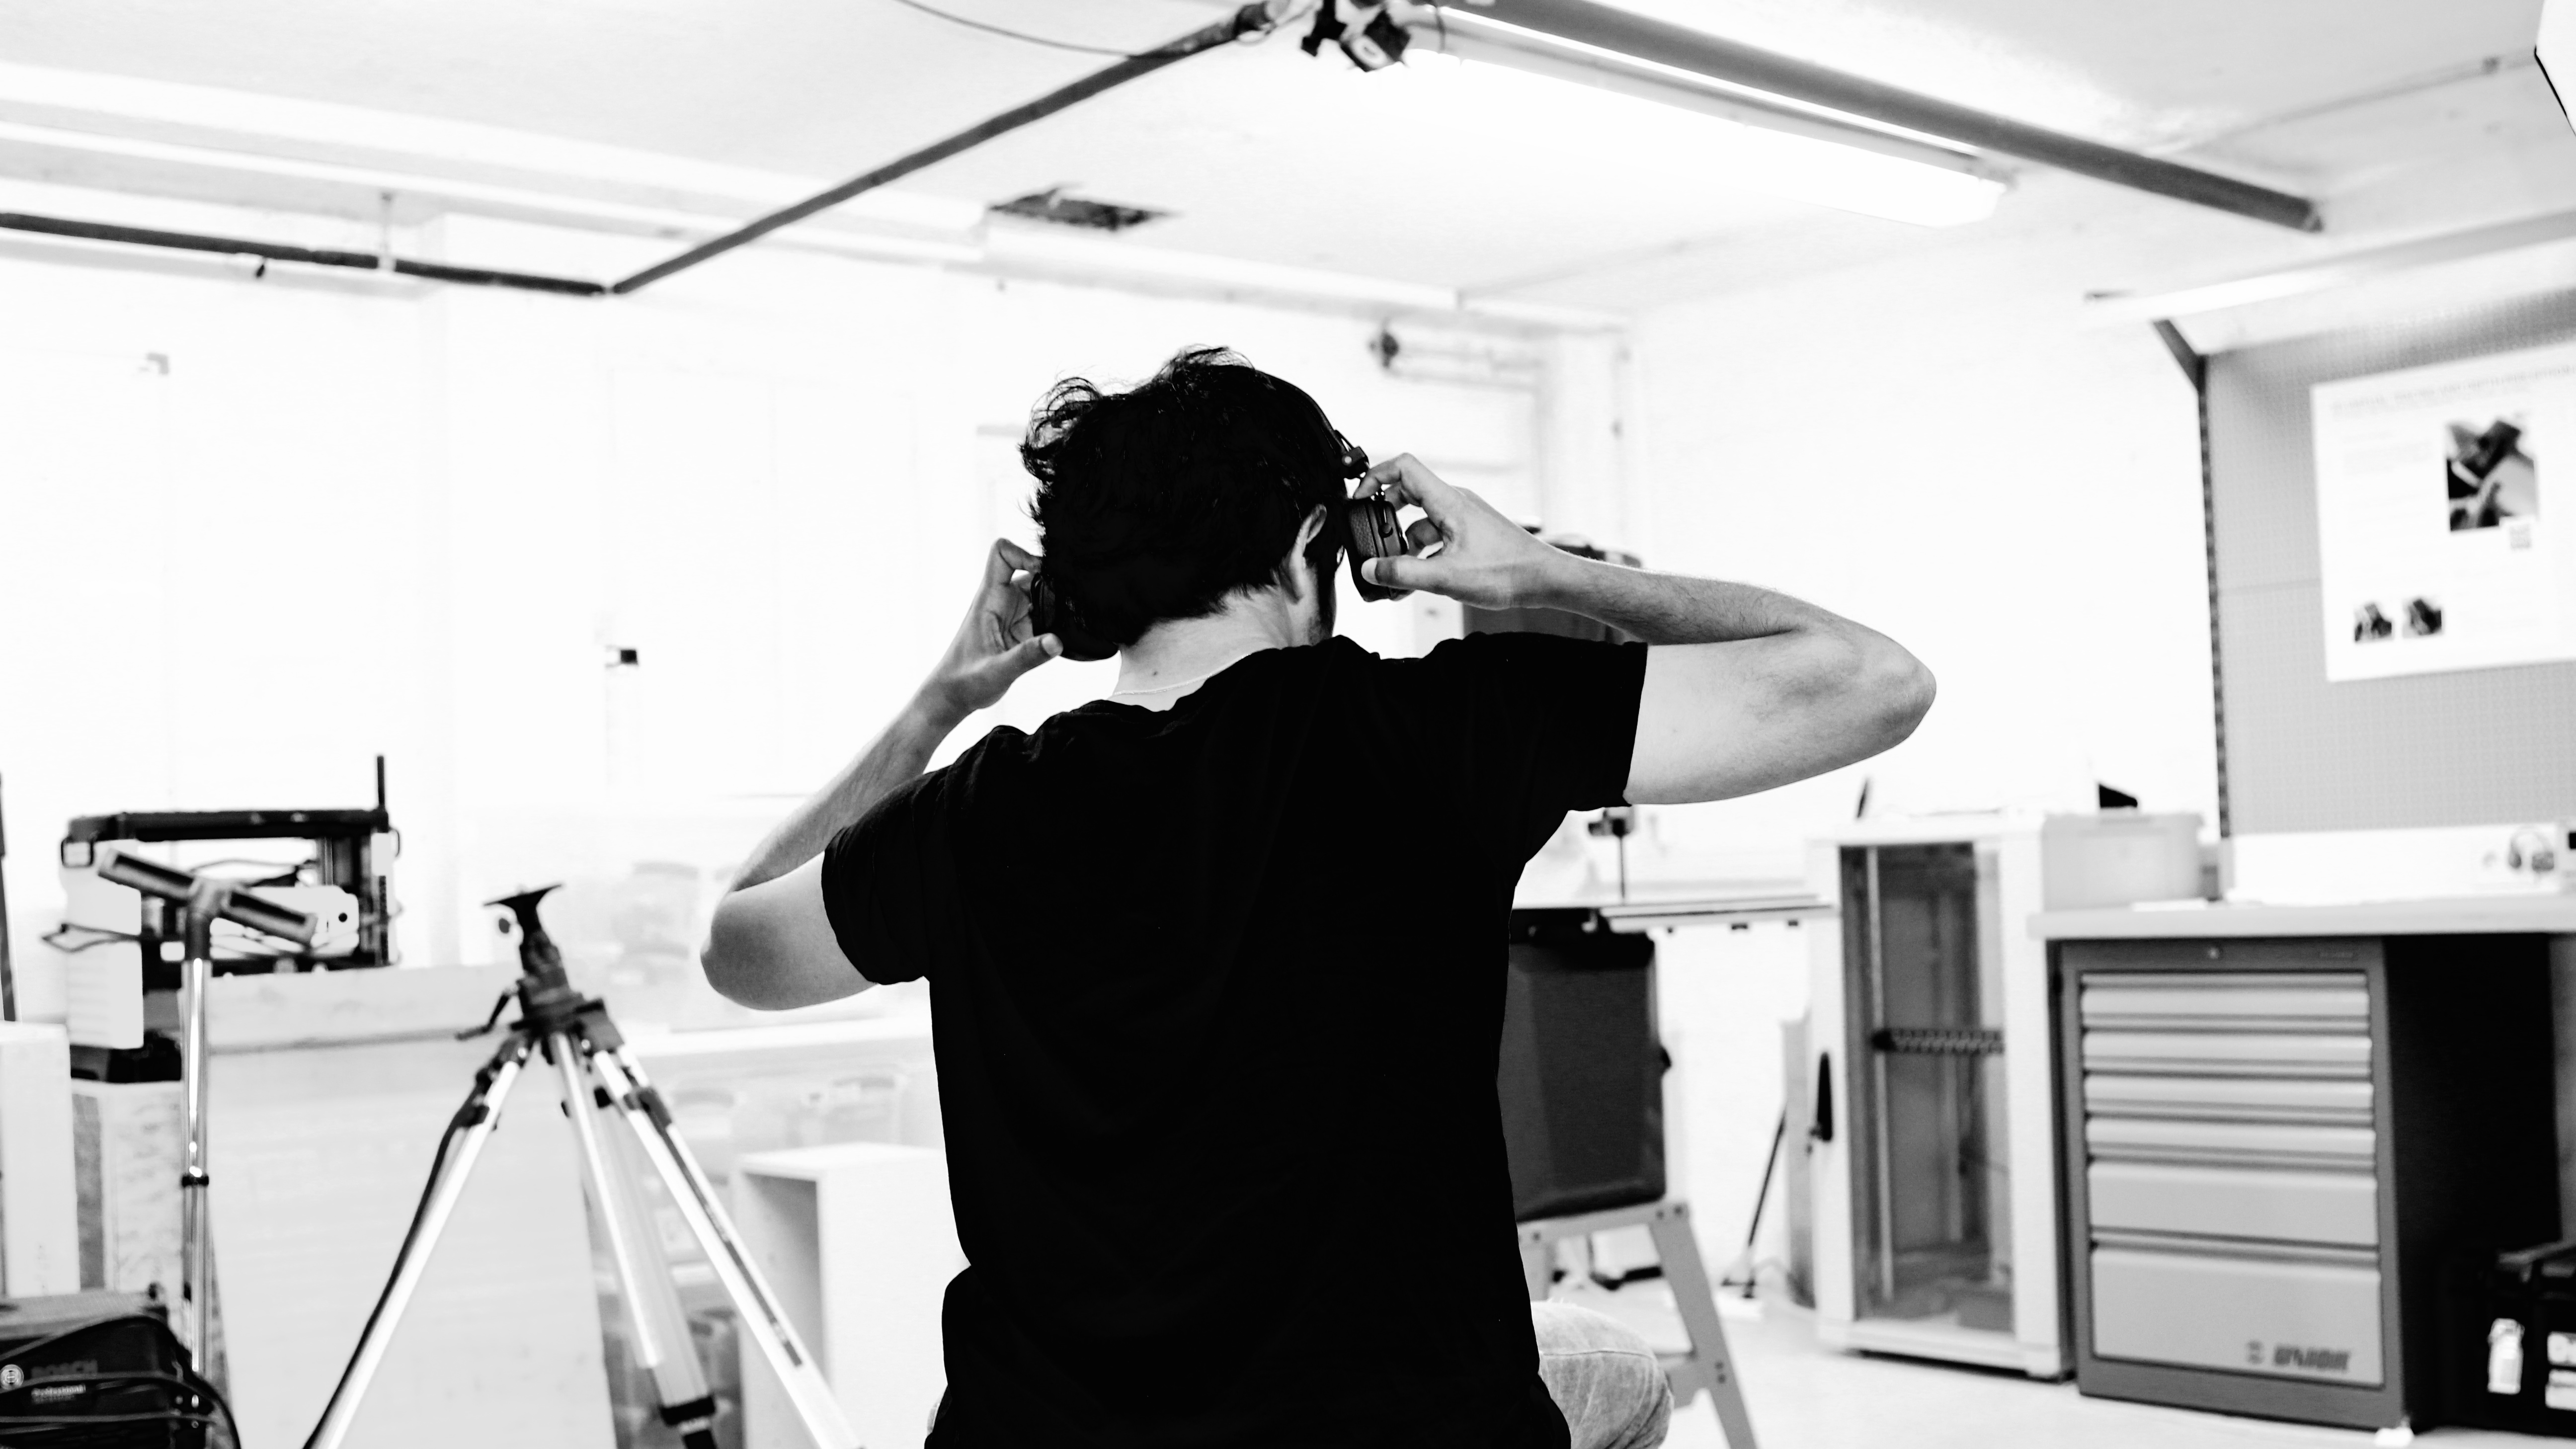
\includegraphics[width=\textwidth]{acmart-master-2/samples/test2bw.png}
  \caption{Concept: We see a future where we no longer need tangible interfaces. Rather humans would let go of these interfaces to give way to a more natural and seamless music interface.}
  \Description{photo of a user removing headphones.}
  \label{fig:teaser}
\end{teaserfigure}
%%
%% This command processes the author and affiliation and title
%% information and builds the first part of the formatted document.
\maketitle

\section{Introduction}
%Humans have been listening to music since 
Humans and music have been existing together for a very long time. According to biologists, the first species of humans developed their first voice box (considered as the first musical instrument), around 530,000 years ago. Not so long after that, the first musical instrument, in the form of a bone flute from 40,000 years ago was uncovered in Central Europe \cite{higham2012tauesting}. Since then, both humans and the instruments they used, have rapidly evolved. As newer technologies are introduced, more ways of creating, producing and even sharing music \cite{voida2005listening} are also taking place. In turn, music has been considered to be culturally universal \cite{campbell1997music, seeger1971reflections} and present across all parts of the globe, reshaping the ways human lived and expressed their emotions \cite{juslin2001music}.

Experts believe that music originated from naturally occurring sounds and rhythms and humans echo them using patterns, making repetitions and considering tonality. In prehistoric and ancient times, humans first created music by blowing wind pipes which are now known as wind instruments \cite{conard2009female}. In the classical and renaissance eras, guitars with strings that can be strummed, piano with keys that can be pressed, cymbals made of metal that can be slammed against each other, were used by humans to create sound. The atomic era and the introduction of the silicon led to MIDI interfaces, electric guitars and synthesizers; devices made of circuits that recreate traditional music instruments, and can be connected to the computer. Now, the information era has led to the development of algorithms, information retrieval (MIR) and artificial intelligence (AI) techniques that allowed humans to work with computers in creating new content. This also introduced social platforms that allowed humans to share and appreciate musical content. As more technological innovations are introduced, humans have also evolved on how they interact with music. 

This paper attempts to share the authors' visions of how humans create, share and interact with music in the future eras. We present our position based on the trends on (1) how musical instruments have evolved, (2) how humans have used them and (3) how can we go back to a more natural but technologically-empowered musical experiences? We present 3 distinct scenarios where our natural musical interface can be best applied. Lastly, we present questions and challenges that provoke discussions involving usability, security, intellectual property and many other relevant key topics on music. 
% styles and types of music 
% instruments
% recent innovations in music, IR, AI 

%\section{Background}
%paragraph 1: Humans instint of safety and the role of music 
%paragraph 2: trends of how music instruments have evolved

\section{Re-imagining the music interface}
% paragraph 1: music an experience that you can be immersed in without losing touch of reality
Recent innovations have attempted to address open problems in music. We use AI techniques to help humans compose music [semi-]automatically; use MIR algorithms to help composers express their emotions and use AR to make immersive music experiences. We envision the future of a music interface that combines all these innovations into a natural interface. We present two ways on how we re-imagined them: 

\begin{figure}[h]
  \centering
  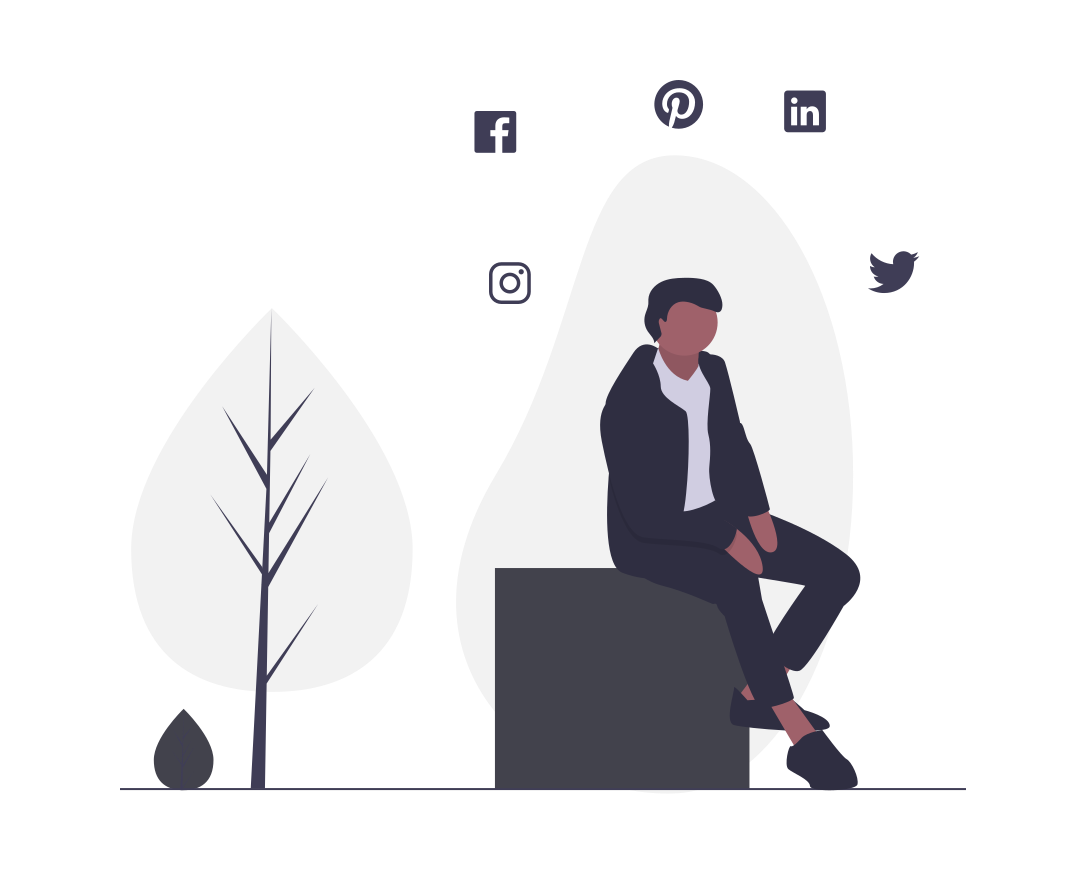
\includegraphics[width=\linewidth]{acmart-master-2/samples/thinkbnw.png}
  \caption{Concept: Humans do not need wide boards, mobile devices, or digital walls. Ideas and concepts are conceived mentally and are interpreted into \textit{"reality"} as musical or creative instructions by algorithms present in a global neurological interface. }
  \Description{Figure of a person thinking and not touching anything.}
  \label{fig: think}
\end{figure}

\textit{Music is an experience that you can be immersed in without losing touch of reality}. Many people believe that the future will be a world where distinguishing reality from the virtual would be challenging \cite{tamura2001mixed}. However, we believe that the future will be its exact opposite. Society will come to a point where it will halt its transition to going completely-virtual but rather, take a step back and move towards going more natural. One of the primary instincts of humans is survival \cite{khantzian1983self}. As such, innovations will push towards sustainability - this includes the development of environments and spaces with less carbon footprint but with swifter technological infrastructure. We envision a future where objects will not have brutalist or neo-futuristic designs. Rather, we see a future of natural objects that are connected to the cloud where it has access to superb computing power. These objects, are our typical things we see in our natural surroundings, but equipped with special nano-chips that allow them to be part of the global link of information; capable of moving themselves depending on the needed use. These chips allow our natural objects to be part of a global network where, humans are a part of through a neurological interface. Thereby allowing humans and objects to telepathically-communicate. 

Looking at the trends of how humans created music:  they pressed two stones against each other to produce basic rhythms and sounds. They began developing instruments with parts, keys and buttons that can be pressed to produce sounds and synths. In any approach, humans transferred their creative thoughts unto the interface of these instruments through a pressing/hitting motion. In the future we envision, humans can feel their emotions and these will be amplified by the music naturally produced by the objects surrounding them. No more pressing, hitting, strumming or the like (see Fig \ref{fig: think}. Algorithms design and produce rhythms in real-time and have them played via vibration by these nearby objects (moving on their own). If humans pressed buttons in the past, humans will simply need to think of these emotions and sounds, and the objects near them will seamlessly produce the vibrations recreating these sounds. Humans will get to enjoy their favorite tunes through this natural interface where instructions and processes are communicated through this neurological link online. We believe that through this neurological interface, humans can create and experience music without losing touch of reality. Humans can perform their daily tasks and be able to seamlessly enjoy the music they hear, produced by the objects around them without having to move a single muscle in their bodies. 

\textit{Music as a gateway for human emotions}. Traditionally, there are two ways on how music becomes a gateway for our emotions. If we feel sad, we wish to hear music so we can reflect, dive deeper and understand the sadness that we feel [emotions going in]. This experience gives us lessons on how to manage our emotions, and how to be stronger. At times, we may feel sad so we wish to hear music in order to improve our mood [emotions going out] and spend the better part of our days. Through our natural and seamless interface, humans can create gateways for their emotions with music. As humans are connected to the global highway of information, unobtrusive sensors no longer need to detect and distinguish the current affect that they feel. Because of their neurological connection to the world, their emotions are easily read and \textit{felt} by the objects around them. Similar to how empathetic spaces that are context and emotion aware, objects nearby will be act as local producers of music to either amplify or address the emotions that humans are feeling. 
% gateway cos two way in and out 
%\textit{We create music because of the emotions we wish to express}. Sentence here. 
% music to express/share
% i am heartbroken when i hear some song i can get to understand more what im feeling
% this music blends with my emotion and it amplifies 
% i am a musician i am expressing my feelings with music 
% music comes from emotions and we create music to retain, continue experiencing these emotions
% 
\section{Design Scenarios}
To better explain how we re-imagined this natural music interface, we propose design scenarios. In these events, we describe how our vision is implemented based on different parameters and conditions. First we imagine being able to listen to music while performing wet activities (such as surfing, scuba diving, etc) without the need for waterproof music gear. Second, we imagine humans being able to listen to music in vacuum spaces such as outer space. We also utilize \textit{the sound of planets, stars and galaxies} as objects to create music from their vibrations. Third, we present a scenario where humans can easily augment their emotional experiences using music with the blink of an eye. 

\begin{figure}[h]
  \centering
  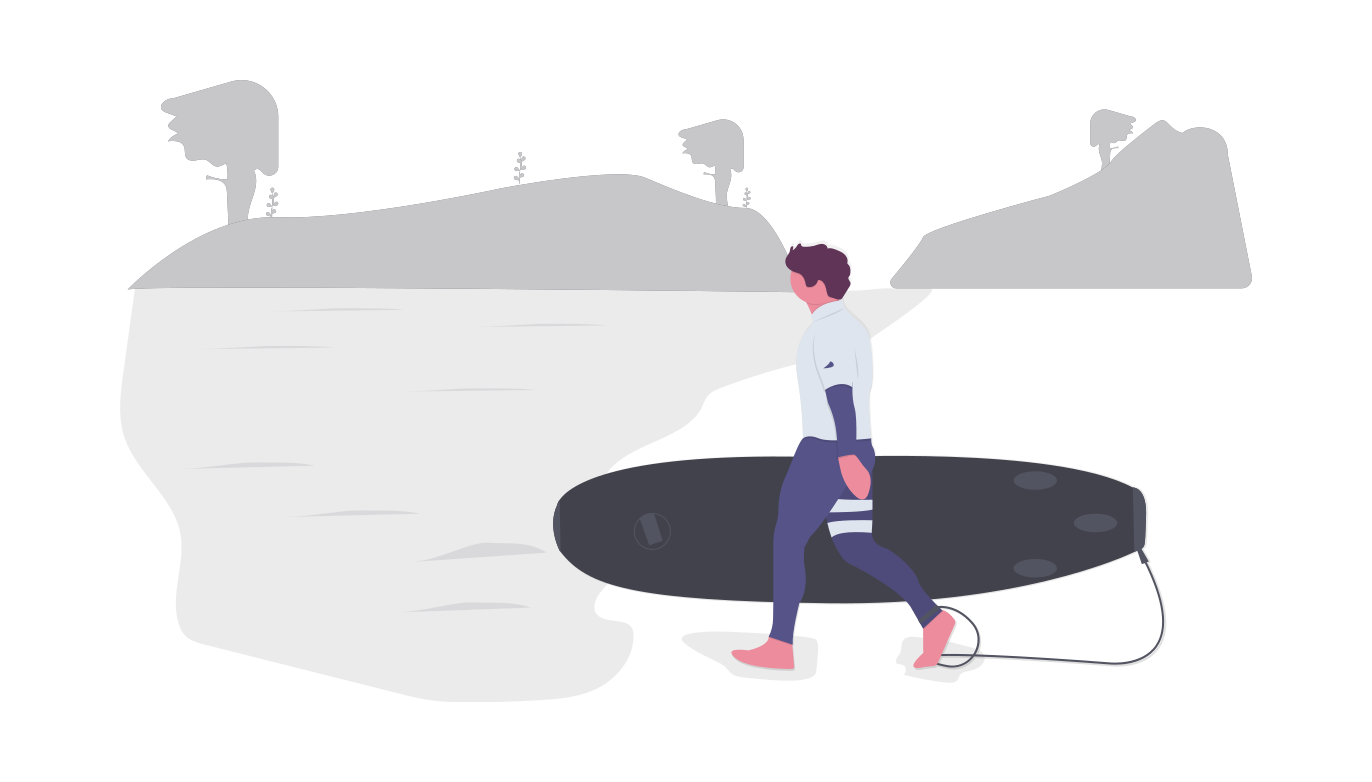
\includegraphics[width=\linewidth]{acmart-master-2/samples/surfbnw.png}
  \caption{Concept: Listening to music while surfing in the wide ocean will no longer require waterproof music gear. Rather, natural elements that are interlinked together create vibrations that humans can hear. Humans can finally achieve a non-obtrusive way of listening music while enjoying their wet hobbies. }
  \Description{Figure of a surfer headed to the sea listening to music without the need of special gear.}
  \label{fig: surf}
\end{figure}
% scenario : swimming in corals/alone in the forest. describe tech. add photos
\textit{No need to add background music in watersport videos; you listen to them as you surf}. NUWAN, add your scenario here. Something like "It is a perfect sunny day. The wind blows nice, and the water is just right. Cuauhtli decides it is the perfect time to go surfing (as seen in Fig \ref{fig: surf}). He prefers to feel this adrenaline rush with the sound of rock music in his ears.... 


% scenario: algorithms that easily convert our emotion stimuli into actual music
\textit{Creating music from vacuum spaces using the sound of space}. Sentence here. 
NUWAN also add your stuff here. Like the previous scenario. 

% discovering new music 
\textit{Amplifying emotions at the blink of an eye}. Sentence here. 
NUWAN also here. 


\section{Conclusion}
The visions and scenarios we presented come with their respective issues and challenges in implementation and in policy design. If we imagine a natural and seamless interface, evaluating its usability will introduce a new paradigm for HCI researchers. Will existing models such as Fitts' Law (which has always worked on any interface developed - mechanical, digital, virtual) still work in neurological links managed by our seamless thoughts? The intangible interaction provided by this \textit{"online network"} could potentially blur concepts such as piracy and intellectual property. As music is composed by ubiquitous algorithms connected to our personal thoughts and feelings, are all our emotions and the music that are generated by them considered unique? shareable? These among many others are interesting questions that we leave to our readers as we re-imagined a natural music interface. While these visions appear to be very far from reality, we are only left with our own thoughts to begin with and maybe hopefully in the not so near future too. 

%%
%% The next two lines define the bibliography style to be used, and
%% the bibliography file.
\bibliographystyle{ACM-Reference-Format}
\bibliography{sample-base}

\end{document}
\endinput
%%
%% End of file `sample-acmtog.tex'.
